\pgfplotsset{
  kernel-axis/.style = {
    domain = -1:1,
    legend pos = north east,
    axis x line = middle,
    axis y line = middle,
    samples = 50,
    xtick = {-1, 1},
    scale only axis
  }
}

\pgfplotsset{kernel/.style = {very thick}}
\pgfplotsset{nabla/.style = {solid, blue}}
\pgfplotsset{laplace/.style = {dashed, red}}


\section{Метод гидродинамики сглаженных частиц}
\subsection{Интегральная аппроксимация функции}
Представление функций распределения физических величин в методе сглаженных частиц опирается на интегральное представление функции:
\begin{equation}
  f(\vect r)=\int\limits_\Omega f(\vect{\tilde r})\delta(\vect r-\vect{\tilde r})d\vect{\tilde r},
\end{equation}
\begin{conditions}
  $f$ & непрерывная функция радиус-вектора $\vect r$;\\
  $\Omega$ & объём, содержащий точку $\vect r$;\\
  $\delta$ & дельта-функция Дирака:
\end{conditions}
\begin{equation}
  \delta(\vect r)=
  \begin{cases}
    +\infty, & \vect r=0, \\
    \quad 0, & \vect r\neq0
  \end{cases}
\end{equation}

Первым приближением в методе сглаженных частиц является аппроксимация интегрального представления функции путём замены дельта-функции $\delta(\vect r-\vect{\tilde r})$ на функцию $\kernel(\vect r-\vect{\tilde r}, h)$, называемую ядром сглаживания:
\begin{equation} \label{eq:approx-f-int}
  f(\vect r)\approx\approxval{f(\vect r)}=\int\limits_\Omega f(\vect{\tilde r})\kernel(\vect r-\vect{\tilde r}, h)d\vect{\tilde r},
\end{equation}
\begin{conditions}
  $\approxval{\cdot}$ & приближённое значение;\\
  $h$ & радиус сглаживания, определяющий область влияния ядра.
\end{conditions}

Ядро сглаживания должно аппроксимировать дельта-функцию Дирака, то есть
\begin{equation}
  \lim_{h \to 0}\kernel(\vect r-\vect{\tilde r}, h)=\delta(\vect r-\vect{\tilde r})
\end{equation}

\begin{equation}
  \kernel(\vect r-\vect{\tilde r}, h)\geq 0
\end{equation}

Рассмотрим погрешность данной аппроксимации. Для этого воспользуемся разложением в ряд Тейлора в окрестности точки $\vect r$ для дифференцируемой функции $f$:
\[ f(\vect{\tilde r})=f(\vect r)+\nabla f(\vect r)\cdot(\vect{\tilde r} - \vect r)+O(|\vect{\tilde r}-\vect r|^2) \]

Подставляя в (\ref{eq:approx-f-int}), получим:
\begin{align*}
  \approxval{f(\vect r)}&=\int\limits_\Omega\Big[f(\vect r)+\nabla f(\vect r)\cdot(\vect{\tilde r} - \vect r)+O(|\vect{\tilde r}-\vect r|^2)\Big]\kernel(\vect r-\vect{\tilde r}, h)d\vect{\tilde r}\\
  &=f(\vect r)\int\limits_\Omega\kernel(\vect r-\vect{\tilde r}, h)d\vect{\tilde r}\\
  &+\nabla f(\vect r)\cdot\int\limits_\Omega(\vect{\tilde r}-\vect r)\kernel(\vect r-\vect{\tilde r}, h)d\vect{\tilde r}\\
  &+\int\limits_\Omega O(|\vect{\tilde r}-\vect r|^2)\kernel(\vect r-\vect{\tilde r}, h)d\vect{\tilde r}
\end{align*}

Для упрощения первого слагаемого введём условие нормировки
\begin{equation}
  \int\limits_\Omega\mathbb W(\vect r-\vect{\tilde r}, h)d\vect{\tilde r}=1
\end{equation}

Для упрощения второго слагаемого введём условие чётности
\begin{equation}
  \kernel(\vect r-\vect{\tilde r}, h)=\kernel(\vect{\tilde r}-\vect r, h)
\end{equation}

Для упрощения третьего слагаемого введём условие финитности
\begin{equation}
  \kernel(\vect r-\vect{\tilde r}, h)=0,\;\text{для}\;|\vect r-\vect{\tilde r}|>h
\end{equation}

И, следовательно,
\begin{equation}
  \approxval{f(\vect r)}=f(\vect r)+O(h^2)
\end{equation}

Таким образом, погрешность данной аппроксимации имеет второй порядок.

Сглаживающая функция $\kernel(\vect r-\vect{\tilde r}, h)$ имеет большое значение, и от её выбора зависит аппроксимация решения в численном методе. Форма ядра задаёт степень взаимного влияния соседних частиц.

За время развития метода исследователями были предложены различные сглаживающие ядра, а также разработана методика получения подобных ядер \cite{liu}.


\subsection{Аппроксимация полей и их производных по частицам}
Теперь, имея интегральную аппроксимацию функции, полученную с помощью сглаживающего ядра, можно перейти к аппроксимации на дискретном наборе частиц, на которые разбивается моделируемая среда, со своими дискретными значениями функции $f(\vect r_i)$.

В процессе подобной дискретизации интегралы могут быть заменены суммирование по соседним частицам, лежащим в носителе сглаживающей функции в данной точке. При этом бесконечно малый объём $d\vect{\tilde r}$ около положения $j$ частицы заменяется на конечный объём частицы $V_j$ и вводится её масса
\begin{equation}
  m_j=V_j\rho_j,
\end{equation}
где $\rho_j$~--- плотность частицы $j$.

Преобразуем уравнение приближённого значения:
\begin{align*}
  \approxval{f(\vect r)}&=\int\limits_\Omega f(\vect{\tilde r})\kernel(\vect r-\vect{\tilde r}, h)d\vect{\tilde r}\\
  &\approx\sum_{j=1}^N f(\vect r_j)\kernel(\vect r-\vect r_j, h)V_j\\
  &=\sum_{j=1}^N f(\vect r_j)\kernel(\vect r-\vect r_j, h)\frac{m_j}{\rho_j},
\end{align*}
где $N$~--- кол-во частиц в рассматриваемом носителе.

Таким образом, приближённое значение поля в $j$ частице определяется как
\begin{equation} \label{eq:approx-f}
  f(\vect r_i)\approx\sum_{j=1}^N\frac{m_j}{\rho_j}f(\vect r_j)\kernel(\vect r_i-\vect r_j, h)
\end{equation}

\begin{figure}[h]
  \centering
  \includegraphics[width=\textwidth]{particle-approx.png}
  \caption{Аппроксимация по частицам}
\end{figure}

В уравнения, описывающие моделируемую среду (\ref{eq:momentum}), кроме самих физических величин входят также их пространственные первые и вторые производные, поэтому необходимо иметь возможность аппроксимировать градиенты и лапласианы этих функций.

\begin{align*}
  \nabla\bigg(\frac{m_j}{\rho_j}f(\vect r_j)\kernel(\vect r_i-\vect r_j, h)\bigg)&=\nabla\bigg(\frac{m_j}{\rho_j}f(\vect r_j)\bigg)\kernel(\vect r_i-\vect r_j, h)\\
  &+\frac{m_j}{\rho_j}f(\vect r_j)\nabla\bigg(\kernel(\vect r_i-\vect r_j, h)\bigg)\\
  \cong 0\cdot \kernel(\vect r_i-\vect r_j, h)&+\frac{m_j}{\rho_j}f(\vect r_j)\nabla\bigg(\kernel(\vect r_i-\vect r_j, h)\bigg),
\end{align*}
где $\nabla\Big(\frac{m_j}{\rho_j}f(\vect r_j)\Big)\cong 0$, поскольку значение в точки $j$ слабо зависит от координаты $\vect r$ и может быть принято постоянной величиной.

Таким образом, приближённое значение градиента поля в $j$ частице
\begin{equation} \label{eq:approx-nabla-f}
  \nabla f(\vect r_i)\approx\sum_{j=1}^N\frac{m_j}{\rho_j}f(\vect r_j)\nabla\kernel(\vect r_i-\vect r_j, h)
\end{equation}

Выражение для лапласиана записывается как
\begin{equation} \label{eq:approx-laplace-f}
  \laplace f(\vect r_i)\approx\sum_{j=1}^N\frac{m_j}{\rho_j}f(\vect r_j)\laplace\kernel(\vect r_i-\vect r_j, h)
\end{equation}

Однако также используется <<симметризованный>> вариант аппроксимации градиента \cite{monaghan}:
\begin{equation} \label{eq:approx-sym-nabla-f}
  \nabla f(\vect r_i)\approx\rho_i\Bigg(\sum_{j=1}^N m_j\bigg(\frac{f(\vect r_j)}{\rho_j^2}+\frac{f(\vect r_i)}{\rho_i^2}\bigg)\nabla\kernel(\vect r_i-\vect r_j, h)\Bigg)
\end{equation}

Одним из важнейших отличий данных приближений является то, что значение функции $f$ входят в них в форме парных частиц, что даёт более точные результаты при моделировании \cite{monaghan}.

Получается, что представление в методе ГСЧ позволяет определить градиент поля по его значению и градиенту сглаживающей функции $\kernel$ вместо дифференцирования функции распределения поля.


\subsection{Резюме}
\begin{enumerate}
  \item Метод ГСЧ является методом интерполяции, который может аппроксимировать непрерывные поля и их производные с помощью дискретных точек, называемых частицами.
  \item Частицы обладают массой $m$, позицией $\vect r$ и скоростью $\vect u$, но могут также содержать расчётные величины, например плотность $\rho$, давление $p$ и так далее.
  \item Связь массы, плотности и объёма определяется как $V=\frac{m}{\rho}$.
  \item Сглаживающая функция должна:
    \begin{enumerate}
      \item аппроксимировать дельта-функцию: $lim_{h \to 0}\kernel(\vect r-\vect{\tilde r}, h)=\delta(\vect r-\vect{\tilde r})$
      \item быть неотрицательной: \quad $\kernel(\vect r-\vect{\tilde r}, h)\geq 0$
      \item быть нормированной: \quad $\int_\Omega\mathbb W(\vect r-\vect{\tilde r}, h)d\vect{\tilde r}=1$
      \item быть чётной: \quad $\kernel(\vect r-\vect{\tilde r}, h)=\kernel(\vect{\tilde r}-\vect r, h)$
      \item обладать финитностью: $\kernel(\vect r-\vect{\tilde r}, h)=0, \;\text{для}\; |\vect r-\vect{\tilde r}|>h$
    \end{enumerate}
  \item Формулы аппроксимации для частиц:
    \begin{enumerate}
      \item $f(\vect r_i)\approx\sum_{j=1}^N\frac{m_j}{\rho_j}f(\vect r_j)\kernel(\vect r_i-\vect r_j, h)$
      \item $\nabla f(\vect r_i)\approx\sum_{j=1}^N\frac{m_j}{\rho_j}f(\vect r_j)\nabla\kernel(\vect r_i-\vect r_j, h)$
      \item $\laplace f(\vect r_i)\approx\sum_{j=1}^N\frac{m_j}{\rho_j}f(\vect r_j)\laplace\kernel(\vect r_i-\vect r_j, h)$
      \item $\nabla f(\vect r_i)\approx\rho_i\Big(\sum_{j=1}^N m_j\big(\frac{f(\vect r_j)}{\rho_j^2}+\frac{f(\vect r_i)}{\rho_i^2}\big)\nabla\kernel(\vect r_i-\vect r_j, h)\Big)$
    \end{enumerate}
  \item ГСЧ применим для задач с сжимаемыми жидкостями и газами.
\end{enumerate}


\section{Гидродинамика Лагранжа}
Использование метода частиц вместо сеток позволяет избавится от уравнения неразрывности (\ref{eq:continuity}), так как количество частиц фиксировано на время моделирования, а масса закреплена за каждой частицей, то уравнение выполняется автоматически.

Заметим, что
\begin{align}
  \begin{split}
    \frac{d}{dt}\vect u\big(t, \vect r(t)\big)&=\frac{\partial\vect u}{\partial t}+\frac{\partial\vect u}{\partial x}\frac{\partial x}{\partial t}+\frac{\partial\vect u}{\partial y}\frac{\partial y}{\partial t}+\frac{\partial\vect u}{\partial z}\frac{\partial z}{\partial t}\\
    &=\frac{\partial\vect u}{\partial t}+\bigg(\frac{\partial\vect u}{\partial x}, \frac{\partial\vect u}{\partial y}, \frac{\partial\vect u}{\partial z}\bigg)\cdot\bigg(\frac{\partial x}{\partial t}, \frac{\partial y}{\partial t}, \frac{\partial z}{\partial t}\bigg)\\
    &=\frac{\partial\vect u}{\partial t}+\Bigg(\vect u\cdot\bigg(\frac{\partial}{\partial x}, \frac{\partial}{\partial y}, \frac{\partial}{\partial z}\bigg)\!\Bigg)\vect u\\
    &=\bigg(\frac{\partial}{\partial t}+\vect u\cdot\nabla\bigg)\vect u
  \end{split}
\end{align}

А, значит, уравнение движения (\ref{eq:momentum}) можно записать как
\begin{equation} \label{eq:lagrange}
  \rho\frac{d\vect u}{dt}=-\nabla p+\mu\laplace\vect u+\vect f
\end{equation}

Правая часть уравнения состоит из внутренних и внешних объёмных сил, $\vect F=-\nabla p+\mu\laplace\vect u+\vect f$. Для частицы $i$ ускорение принимает вид
\begin{equation} \label{eq:acceleration}
  \vect a_i=\frac{d\vect u_i}{dt}=\frac{\vect F_i}{\rho_i}
\end{equation}

Если не указано другое, то в качестве сглаживающего ядра будем использовать предложенное в \cite{muller}
\begin{equation}
  \kernel_d(\vect r, h)=\frac{315}{64\pi h^9}
  \begin{cases}
    \left(h^2-|\vect r|^2\right)^3, & 0\leq|\vect r|\leq h, \\
    \qquad 0, & h<|\vect r|
  \end{cases}
\end{equation}

\begin{figure}
  \centering
  \resizebox{.5\textwidth}{!} {
    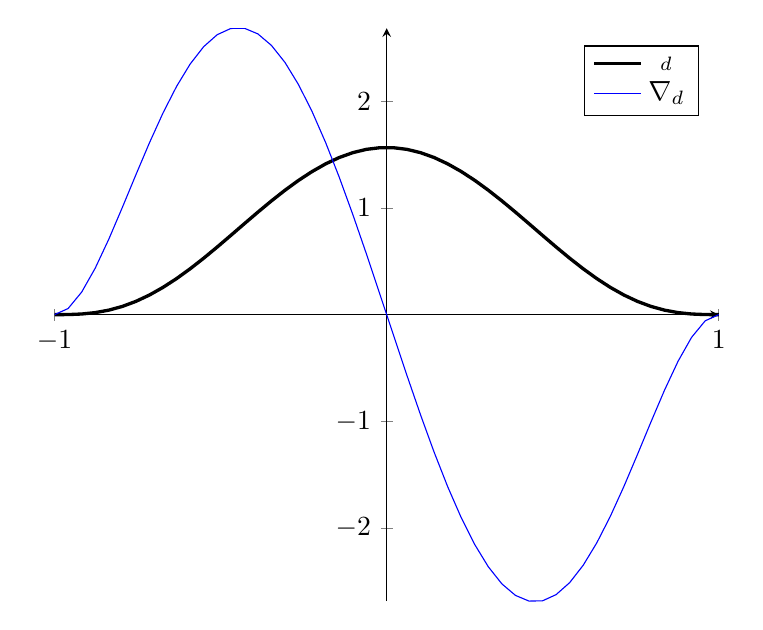
\begin{tikzpicture}
      \begin{axis}[kernel-axis]
        \legend{$\kernel_d$, $\nabla\kernel_d$}
        \addplot[kernel]{315/(64*pi)*(1-x^2)^3};
        \addplot[nabla]{-945/(32*pi)*x*(1-x*x)^2};
      \end{axis}
    \end{tikzpicture}
  }%
  \resizebox{.5\textwidth}{!} {
    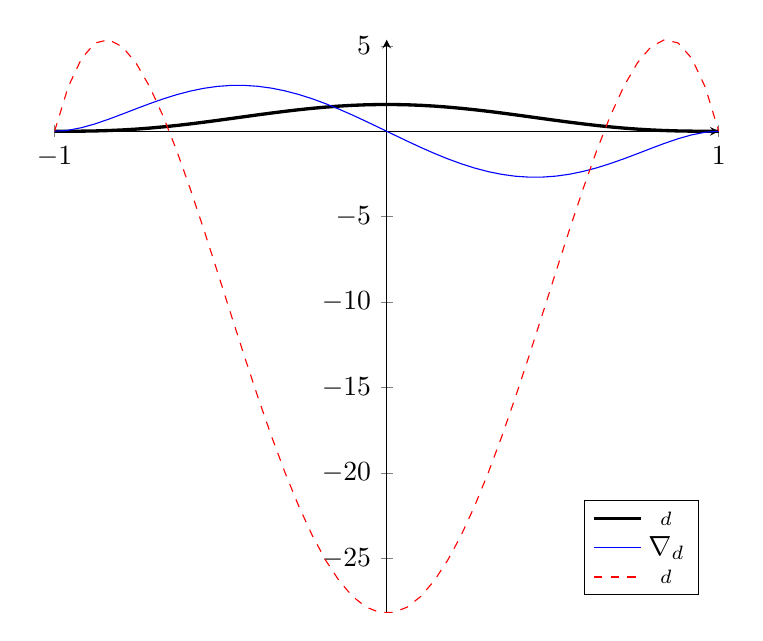
\begin{tikzpicture}
      \begin{axis}[kernel-axis, legend pos = south east]
        \legend{$\kernel_d$, $\nabla\kernel_d$, $\laplace\kernel_d$}
        \addplot[kernel]{315/(64*pi)*(1-x^2)^3};
        \addplot[nabla]{-945/(32*pi)*x*(1-x*x)^2};
        \addplot[laplace]{-945/(32*pi)*(1-x*x)*(3 - 7*x*x)};
      \end{axis}
    \end{tikzpicture}
  }
  \caption{Стандартное сглаживающее ядро при $h=1$.}
  \label{fig:kernel-default}
\end{figure}


\subsection{Плотность}
Согласно ГСЧ любое непрерывное значение поля, его градиент и лапласиан могут быть аппроксимированы, используя уравнения (\ref{eq:approx-f}), (\ref{eq:approx-nabla-f}) и (\ref{eq:approx-laplace-f}) соответственно. В уравнениях предполагается, что массы и плотности известны для всех частиц. Так как масса задаётся пользователем, то необходимо предварительно найти только плотности.

Для этого воспользуемся уравнением (\ref{eq:approx-f}) и получим окончательное выражение:
\begin{equation} \label{eq:density}
  \rho_i=\sum_j m_j\kernel_d(\vect r_i-\vect r_j, h)
\end{equation}


\subsection{Давление}
Давление частицы может быть определено, используя уравнение идеального газа
\begin{equation}
  pV=\nu RT,
\end{equation}
\begin{conditions}
  $V$ & объём, $V=\frac{m}{\rho}$;\\
  $\nu$ & количество вещества;\\
  $R$ & универсальная газовая постоянная;\\
  $T$ & температура.
\end{conditions}

Так как мы рассматривает изотермическую жидкость с постоянной массой, то введём константу $k=\frac{\nu}{m}RT$:
\[ \frac{p}{\rho}=k\Rightarrow p=k\rho \]

Однако такой подход приводит к чисто отталкивающим силам между частицами, что справедливо для идеального газа, который имеет тенденцию к расширению в пространстве. В противоположность этому, жидкости обладают внутренней связностью и имеют постоянную плотность в покое. В \cite{desbrun} предлагается использовать модифицированную версию уравнения состояния идеального газа:
\begin{align*}
  (p+p_0)V&=k\\
  p+k\rho_0&=k\rho
\end{align*}
\begin{equation} \label{eq:pressure}
  p=k(\rho-\rho_0),
\end{equation}
где $\rho_0$~--- плотность жидкости в равновесном состоянии.

Так как речь идёт о силе, то использовать стандартное уравнение для аппроксимации градиента функции (\ref{eq:approx-nabla-f}) недостаточно, так как оно асимметрично, а значит третий закон Ньютона не выполняется. Поэтому мы будем использовать симметричное уравнение (\ref{eq:approx-sym-nabla-f}):
\[ \vect f_i^p=-\nabla p(\vect r_i)=-\rho_i\sum_{j\neq i}\left(\frac{p_i}{\rho_i^2}+\frac{p_j}{\rho_j^2}\right)m_j\nabla\kernel(\vect r_i-\vect r_j, h). \]

Использование $\kernel=\kernel_d$ в данном случае является не лучшим выбором, поскольку $\nabla\kernel_d(\vect r, h)\to 0$ при $|\vect r|\to 0$ (рис.~\ref{fig:kernel-default}), что ведёт к кластеризации частиц в регионах с высоким давлением. Поэтому в \cite{desbrun} была предложена другая сглаживающая функция:
\begin{equation}
  \kernel_p(\vect r, h)=\frac{15}{\pi h^6}
  \begin{cases}
    (h-|\vect r|)^3, & 0\leq|\vect r|\leq h\\
    \qquad 0, & h<|\vect r|
  \end{cases}
\end{equation}

\begin{figure}
  \centering
  \resizebox{.5\textwidth}{!} {
    \begin{tikzpicture}
      \begin{axis}[kernel-axis, ymin = -17, ymax = 17]
        \legend{$\kernel_p$, $\nabla\kernel_p$}
        \addplot[kernel]{15/pi*(1-abs(x))^3};
        \addplot[nabla, restrict y to domain = -13.5:inf]{-45/pi*x/abs(x)*(1-abs(x))^2};
      \end{axis}
    \end{tikzpicture}
  }%
  \resizebox{.5\textwidth}{!} {
    \begin{tikzpicture}
      \begin{axis}[kernel-axis, legend pos = south east, ymin = -100]
        \legend{$\kernel_p$, $\nabla\kernel_p$, $\laplace\kernel_p$}
        \addplot[kernel]{15/pi*(1-abs(x))^3};
        \addplot[nabla, restrict y to domain = -inf:13.5]{-45/pi*x/abs(x)*(1-abs(x))^2};
        \addplot[laplace]{-90/(pi*abs(x))*(1-abs(x))*(1-2*abs(x))};
      \end{axis}
    \end{tikzpicture}
  }
  \caption{Сглаживающее ядро для давления при $h=1$.}
  \label{fig:kernel-pressure}
\end{figure}

Градиент которой выражается как
\begin{equation}
  \begin{gathered}
    \nabla\kernel_p(\vect r, h)=-\frac{45}{\pi h^6}\frac{\vect r}{|\vect r|}(h-|\vect r|)^2\\
    \lim_{r\to 0\mp0}\nabla\kernel_p(r, h)=\pm\frac{45}{\pi h^4}
  \end{gathered}
\end{equation}

Что позволяет моделировать отталкивание в областях высокой плотности и притягивание в областях низкой плотности (рис.~\ref{fig:repulse-attractive}).

\begin{figure}[h]
  \centering
  \includegraphics[width=.45\textwidth]{repulse-forces.png}
  \includegraphics[width=.45\textwidth]{attractive-forces.png}
  \caption{Отталкивание и притягивание в зависимости от плотности.}
  \label{fig:repulse-attractive}
\end{figure}

Окончательное уравнение:
\begin{equation} \label{eq:pressure-force}
  \vect f_i^p=-\rho_i\sum_{j\neq i}\left(\frac{p_i}{\rho_i^2}+\frac{p_j}{\rho_j^2}\right)m_j\nabla\kernel_p(\vect r_i-\vect r_j, h)
\end{equation}


\subsection{Вязкость}
Жидкость представляет собой вещество, которое не может противостоять напряжению сдвига и, следовательно, будет течь при деформации. В то же время, когда жидкость течет, молекулы испытывают внутреннее трение, а значит часть кинетической энергии переходит в тепло. Сопротивление текучести называется вязкостью, а соответствующая сила входит в (\ref{eq:lagrange}) в виде $\vect f_i^v=\mu\laplace\vect u(\vect r_i)$, где $\mu$~--- динамическая вязкость, которая уменьшается с увеличением температуры, и растёт с увеличением давления.

Поскольку силы вязкости зависят только от разности скоростей, а не от их абсолютных значений, то простейший способ симметризовать аппроксимацию~--- использовать разность скоростей:
\[ \vect f_i^v=\mu\laplace\vect u(\vect r_i)=\mu\sum_{j}(\vect u_j-\vect u_i)\frac{m_j}{\rho_j}\laplace\kernel(\vect r_i-\vect r_j, h) \]

Возможная интерпретация формулы: частица $i$ ускоряется в направлении относительного движения среды.

Заметим, что лапласиан сглаживающего ядра должен был всюду положительным, то есть $\laplace\kernel(\vect r, h)\geq0$ при $|\vect r|\leq h$. Это необходимо, потому что мы не хотим, чтобы силы, вызванные вязкостью увеличивали относительную скорость, и таким образом вводили нестабильность в систему.

Получается, что стандартное сглаживающее ядро ($\kernel_d$) и ядро для давления ($\kernel_p$) не подходят (рис.~\ref{fig:kernel-pressure}). В \cite{muller} предложено использовать следующее ядро:
\begin{equation}
  \begin{gathered}
    \kernel_v(\vect r, h)=\frac{15}{2\pi h^3}
    \begin{cases}
      -\frac{|\vect r|^3}{2h^3}+\frac{|\vect r|^2}{h^2}+\frac{h}{2|\vect r|}-1, & 0<|\vect r|\leq h\\
      \qquad 0, & h<|\vect r|
    \end{cases}\\
    \lim_{r\to 0}\kernel_v(r, h)=\infty
  \end{gathered}
\end{equation}

Лапласиан которого выражается как
\begin{equation}
  \laplace\kernel_v(\vect r, h)=\frac{45}{\pi h^6}(h-|\vect r|)
\end{equation}

\begin{figure}
  \centering
  \resizebox{.5\textwidth}{!} {
    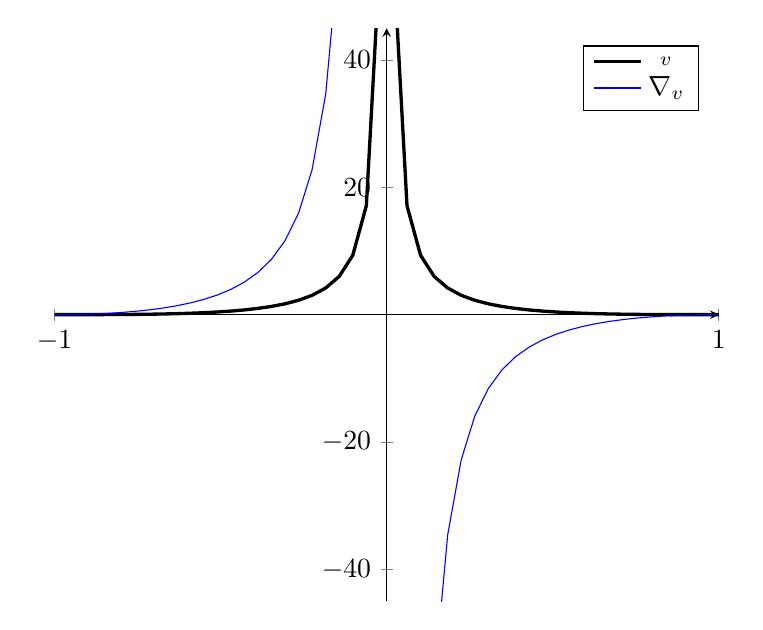
\begin{tikzpicture}
      \begin{axis}[kernel-axis, ymin = -45, ymax = 45]
        \legend{$\kernel_v$, $\nabla\kernel_v$}
        \addplot[kernel]{15/(2*pi)*(-abs(x)^3/2+x*x+1/(2*abs(x))-1)};
        \addplot[nabla, restrict y to domain = -100:100]{15/(2*pi)*x*(-3*abs(x)/2+2-1/(2*abs(x)^3))};
      \end{axis}
    \end{tikzpicture}
  }%
  \resizebox{.5\textwidth}{!} {
    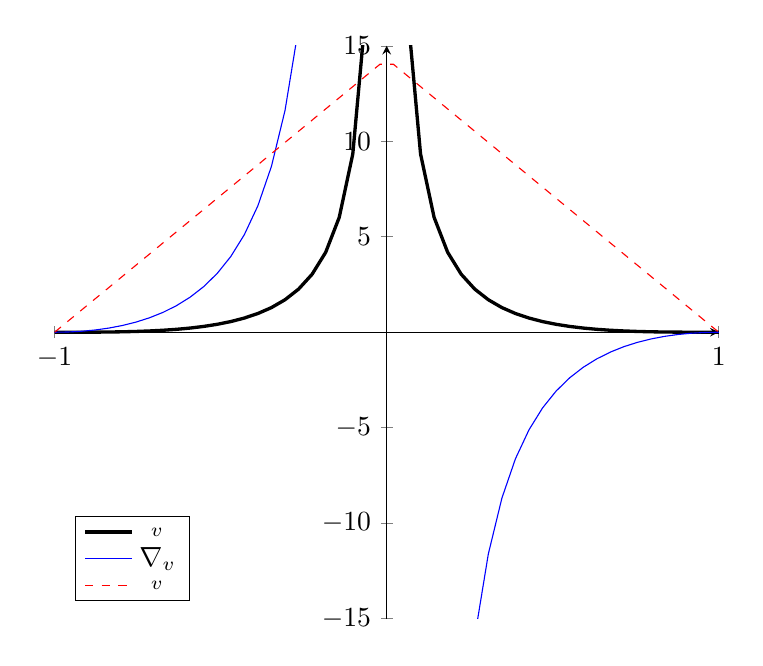
\begin{tikzpicture}
      \begin{axis}[kernel-axis, legend pos = south west, ymin = -15, ymax = 15]
        \legend{$\kernel_v$, $\nabla\kernel_v$, $\laplace\kernel_v$}
        \addplot[kernel]{15/(2*pi)*(-abs(x)^3/2+x*x+1/(2*abs(x))-1)};
        \addplot[nabla, restrict y to domain = -30:30]{15/(2*pi)*x*(-3*abs(x)/2+2-1/(2*abs(x)^3))};
        \addplot[laplace]{45/pi*(1-abs(x))};
      \end{axis}
    \end{tikzpicture}
  }
  \caption{Сглаживающее ядро для вязкости при $h=1$.}
  \label{fig:kernel-viscosity}
\end{figure}

Конечное выражение для сил вязкости:
\begin{equation} \label{eq:viscosity-force}
  \vect f_i^v=\mu\sum_{j}(\vect u_j-\vect u_i)\frac{m_j}{\rho_j}\laplace\kernel_v(\vect r_i-\vect r_j, h)
\end{equation}


\subsection{Внешние силы}
Существуют различные внешние силы, подлежащие моделированию (например, поверхностное натяжение и гравитация). Более того, так как метод является интерактивным, внешние силовые поля также могут быть введены и удалены динамически во время моделирования.

В уравнении (\ref{eq:lagrange}) внешние силы~--- последнее слагаемое, $\vect f$, которое может быть определено как сумма всех полей внешних объёмных сил:
\begin{equation}
  \vect f=\sum_n \vect f^n
\end{equation}

Обработка столкновений, которые также могут рассматривается посредством внешний сил, рассматриваются в следующем разделе отдельно.


\subsubsection{Гравитация}
Гравитация действуют на все частицы:
\begin{equation} \label{eq:gravity-force}
  \vect f_i^g=\rho_i\vect g,
\end{equation}
где $\vect g$~--- ускорение свободного падения.


\subsubsection{Поверхностное натяжение}
Силы поверхностного натяжения являются внешними силами, применяемыми к свободной поверхности жидкой среды. Они, как правило, не является частью уравнений Навье-Стокса, так как считаются граничным условием. Молекулы жидкости находятся под влиянием сил притяжения от соседних молекул, которые уравновешены внутри жидкости. Но на поверхности силы не сбалансированы и вызывают поверхностное натяжение. Эти силы сонаправлены со внутренней нормалью к поверхности жидкости. Силы поверхностного натяжения стремятся сгладить кривизну поверхности (рис.~\ref{fig:tension}).

\begin{figure}[h]
  \centering
  \includegraphics[width=.6\textwidth]{tension.png}
  \caption{Силы поверхностного натяжения.}
  \label{fig:tension}
\end{figure}

Модель для расчёта сил поверхностного натяжения строится на <<цветовой>> функции \cite{muller}:
\[
  c(\vect r) =
  \begin{cases}
    1, & \exists i: \vect r = \vect r_i\\
    0 & \text{иначе}
  \end{cases}
\]

Таким образом,
\begin{equation}
  c_i = c(\vect r_i) = \sum_j\frac{m_j}{\rho_j}\kernel_d(\vect r_i-\vect r_j, h)
\end{equation}

При этом, внутренняя нормаль вычисляется как
\begin{equation} \label{eq:inward-normal}
  \vect n_i=\nabla c(\vect r_i)=\sum_j\frac{m_j}{\rho_j}\nabla\kernel_d(\vect r_i-\vect r_j, h)
\end{equation}

Тогда сила поверхностного натяжения принимает вид
\begin{equation} \label{eq:tension-force}
  \vect f_i^s=-\sigma\laplace c_i\frac{\vect n_i}{|\vect n_i|},
\end{equation}
где $\sigma$~--- коэффициент поверхностного натяжения.

Так как $\frac{\vect n_i}{|\vect n_i|}$ численно нестабильно при $|\vect n_i|\to 0$, необходимо, чтобы частица находилась рядом с поверхностью:
\begin{equation} \label{eq:is-surface}
  |\vect n_i|\geq l,
\end{equation}
где $l>0$~--- некоторая константа предела применения.


\subsection{Обработка столкновений}
Когда частицы сталкиваются с контейнером, они должны оставаться внутри своих границ. Аналогичным образом, если частицы сталкиваются с препятствием, они не могут проникнуть или получить доступ к внутренней части объекта.

Обработка столкновений может быть разделена на два этапа: обнаружение столкновения и реакция на столкновение. В данной работе все препятствия и контейнеры считаются фиксированными и жесткими, следовательно мы будем рассматривать только реакцию на частицы.


\subsubsection{Определение столкновений}
Частицы несут информацию о положении $\vect x$ и скорости, которых достаточно для определения коллизий. Если текущее положение частицы не даёт достаточно информации, чтобы обеспечить правильное соударение, то скорость может быть использована для получения прежней позиции частицы. Обязательная информация о столкновении включает в себя:
\begin{enumerate}
  \item Точка контакта с поверхностью, $\vect{cp}$.
  \item Глубина проникновения, $d$.
  \item Нормаль к поверхности в точке контакта, $\vect n$.
\end{enumerate}

Заметим, что глубина проникновения положительна ($d>0$), то есть нахождение частицы на поверхности объекта не ведёт к  коллизии.

Рассмотрим два возможных определения столкновений (рис.~\ref{fig:two-collisions}): корректное ($\vect{cp}_1$) и упрощённое ($\vect{cp}_2$). Первый более точный, однако последний менее требовательный к вычислительным ресурсам. На практике использование упрощённого варианта не оказывает видимого влияния на симуляцию \cite{kelager}, так как при небольших временных интервалов (рассматриваются в следующей разделе) $d_1\to 0$, а значит и $\vect{cp}_2\to\vect{cp}_1$. Исключение из этого правила составляют небольшие по объёму объекты, однако они в данной работе не рассматриваются.

\begin{figure}[h]
  \centering
  \includegraphics[width=.4\textwidth]{two-collisions.png}
  \caption{Два возможных способа определения столкновений.}
  \label{fig:two-collisions}
\end{figure}

Введём функцию, позволяющую определять положение частицы относительно рассматриваемого объекта:
\begin{equation} \label{eq:test-collision}
  F(\vect x)
  \begin{cases}
    <0, & \text{частица внутри объекта}\\
    =0, & \text{частица на поверхности}\\
    >0, & \text{частица вне объекта}
  \end{cases}
\end{equation}


\subsubsection{Сфера}
Тест на пересечение для сферы записывается как
\begin{equation}
  F_s(\vect x)=|\vect x-\vect c|^2-r^2,
\end{equation}
\begin{conditions}
  $\vect c$ & центр сферы;\\
  $r$ & радиус сферы.
\end{conditions}

Если коллизия имеет место, то точка контакта, глубина проникновения и нормаль к поверхности вычисляется соответственно
\begin{align}
  \vect{cp}_s&=\vect c+r\frac{\vect x-\vect c}{|\vect x-\vect c|}\\
  d_s&=\big||\vect c-\vect x|-r\big|\\
  \vect n_s&=\sgn\big(F_s(\vect x)\big)\frac{\vect c-\vect x}{|\vect c-\vect x|}
\end{align}


\subsubsection{Ограничивающий прямоугольный параллелепипед}
Введём два вспомогательных векторных оператора:
\begin{align*}
  [\vect a]_{abs}:=(|a_x|, |a_y|, |a_z|),\\
  [\vect a]_{max}:=\max(a_x, a_y, a_z)
\end{align*}

Тогда тест на пересечение для ограничивающего прямоугольного параллелепипеда определяется как
\begin{equation}
  F_b(\vect x)=\big[[\vect x']_{abs}-\vect e\big]_{max},
\end{equation}
где $\vect x'$~--- координаты точки $\vect x$ в системе координат параллелепипеда.

\begin{equation}
  \vect x'=(\vect x-\vect c)\vect S^{-1},
\end{equation}
где $\vect S$~--- матрица перехода от мирового базиса к локальному; $\vect c$~--- центр параллелепипеда в мировой системе координат.

Точка пересечения в с.к. параллелепипеда может быть найдена как
\begin{equation}
  \vect{cp}'_b=\min\!\big[\vect e, \max[-\vect e, \vect x']\big],
\end{equation}
а в мировой с.к.
\begin{equation}
  \vect{cp}_b=\vect c+\vect{cp}'_b\vect S
\end{equation}

Тогда глубина проникновения и нормаль:
\begin{align}
  d_b&=|\vect{cp}_b-\vect x|\\
  \vect n_b&=\frac{\sgn[\vect{cp}'_b-\vect x']\vect S }{\big|\sgn[\vect{cp}'_b-\vect x']\vect S\big|}
\end{align}


\subsubsection{Реакция на столкновение}
Когда столкновение обнаружено, необходимо скорректировать позицию частицы и её скорость.
В нашей модели, если частица $i$ проникла через препятствие, то её новая позиция может быть определена как
\begin{equation} \label{eq:correct-position}
  \vect r_i=\vect r_i+d\vect n=\vect{cp}
\end{equation}

Вектор скорости может быть скорректирован согласно отражению для частично упругого столкновения:
\[ \vect u_i=\vect u_i-(1+\beta)(\vect u_i\cdot \vect n)\vect n, \]
где $\beta$~--- коэффициент восстановления, $0\leq \beta\leq1$.

Однако данная модель не идеальна. Так как при столкновении мы имеем дело с частицей, которая уже находится внутри препятствия, то данное уравнение может неправомерно увеличить кинетическую энергию частицы. Мы стремимся моделировать столкновение частицы с импульсом точно по времени, когда произошло столкновение. В \cite{kelager} предлагается использовать для этого временную корректировку:
\begin{equation} \label{eq:correct-velocity}
  \vect u_i=\vect u_i-(1+\beta\frac{d}{\Delta t|\vect u_i|})(\vect u_i\cdot \vect n)\vect n
\end{equation}


\subsection{Численное интегрирование времени}
Во время моделирования используется глобальное фиксированное интервал $\Delta t$. После вычисления ускорения (\ref{eq:acceleration}), позиция частиц может быть получена интегрированием ускорения. Согласно \cite{kelager}, для гидродинамики сглаженных частиц лучше всего показывает себя метод <<чехарды со средней точкой>> (рис.~\ref{fig:leapfrog}):
\begin{align}
  \label{eq:update-velocity}
  \vect u_{t+\frac{1}{2}\Delta t}&=\vect u_{t-\frac{1}{2}\Delta t}+\Delta t\vect a_t,\\
  \label{eq:update-position}
  \vect r_{t+\Delta t}&=\vect r_t+\Delta t\vect u_{t+\frac{1}{2}\Delta t},
\end{align}
с начальным смещением скорости
\begin{equation} \label{eq:init-leapfrog}
  \vect u_{-\frac{1}{2}\Delta t}=\vect u_0-\frac{1}{2}\Delta t\vect a_0
\end{equation}

\begin{figure}[h]
  \centering
  \includegraphics[width=.75\textwidth]{leapfrog.png}
  \caption{Метод <<чехарды со средней точкой>>.}
  \label{fig:leapfrog}
\end{figure}

Скорость для времени $t$ может быть получена как
\begin{equation} \label{eq:current-velocity}
  \vect u_t\approx\frac{\vect u_{t-\frac{1}{2}\Delta t}+\vect u_{t+\frac{1}{2}\Delta t}}{2},
\end{equation}
которое требуется при расчёте сил для времени $t$.


\subsection{Резюме}

\begin{enumerate}
  \item Ускорение частицы под действием объёмных сил $\vect a_i=\frac{d\vect u_i}{dt}=\frac{\vect F_i}{\rho_i}$
  \item Плотность частицы $\rho_i=\sum_j m_j\kernel_d(\vect r_i-\vect r_j, h)$
  \item Внутренняя нормаль к поверхности: $\vect n_i=\sum_j\frac{m_j}{\rho_j}\nabla\kernel_d(\vect r_i-\vect r_j, h)$
  \item Объёмные силы, действующие на частицу, возникают под действием
    \begin{enumerate}
      \item давления $\vect f_i^p=-\rho_i\sum_{j\neq i}\left(\frac{p_i}{\rho_i^2}+\frac{p_j}{\rho_j^2}\right)m_j\nabla\kernel_p(\vect r_i-\vect r_j, h)$
      \item вязкости $\vect f_i^v=\mu\sum_{j}(\vect u_j-\vect u_i)\frac{m_j}{\rho_j}\laplace\kernel_v(\vect r_i-\vect r_j, h)$
      \item гравитации $\vect f_i^g=\rho_i\vect g$
      \item поверхностного натяжения $\vect f_i^s=-\sigma\frac{\vect n_i}{|\vect n_i|} \sum_j\frac{m_j}{\rho_j}\laplace\kernel_d(\vect r_i-\vect r_j, h)    $
    \end{enumerate}
  \item Для обработки столкновения частицы со сферой необходимы
    \begin{enumerate}
      \item тестовая функция $F_s(\vect x)=|\vect x-\vect c|^2-r^2$
      \item точка контакта $\vect{cp}_s=\vect c+r\frac{\vect x-\vect c}{|\vect x-\vect c|}$
      \item глубина проникновения $d_s=\big||\vect c-\vect x|-r\big|$
      \item нормаль $\vect n_s=\sgn\big(F_s(\vect x)\big)\frac{\vect c-\vect x}{|\vect c-\vect x|}$
    \end{enumerate}
  \item Для обработки столкновения с параллелепипедом необходимы
    \begin{enumerate}
      \item тестовая функция $F_b(\vect x)=\big[[\vect x']_{abs}-\vect e\big]_{max}$
      \item точка контакта $\vect{cp}_b=\vect c+\vect{cp}'_b\vect S$, \quad $\vect{cp}'_b=\min\!\big[\vect e, \max[-\vect e, \vect x']\big]$
      \item глубина проникновения $d_b=|\vect{cp}_b-\vect x|$
      \item нормаль $\vect n_b=\frac{\sgn[\vect{cp}'_b-\vect x']\vect S }{\big|\sgn[\vect{cp}'_b-\vect x']\vect S\big|}$, \quad $\vect x'=(\vect x-\vect c)\vect S^{-1}$
    \end{enumerate}
  \item Реакция на столкновение осуществляется путём корректировки
    \begin{enumerate}
      \item положения $\vect r_i=\vect{cp}$
      \item скорости $\vect u_i=\vect u_i-(1+\beta\frac{d}{\Delta t|\vect u_i|})(\vect u_i\cdot \vect n)\vect n$
    \end{enumerate}
  \item Для вычисления положения и скорости используется метод <<чехарды со средней точкой>>:
    \begin{enumerate}
      \item новая скорость $\vect u_{t+\frac{1}{2}\Delta t}=\vect u_{t-\frac{1}{2}\Delta t}+\Delta t\vect a_t$
      \item новое положение $\vect r_{t+\Delta t}=\vect r_t+\Delta t\vect u_{t+\frac{1}{2}\Delta t}$
      \item начальное смещение скорости $\vect u_{-\frac{1}{2}\Delta t}=\vect u_0-\frac{1}{2}\Delta t\vect a_0$
      \item текущая скорость $\vect u_t\approx\frac{\vect u_{t-\frac{1}{2}\Delta t}+\vect u_{t+\frac{1}{2}\Delta t}}{2}$
    \end{enumerate}
\end{enumerate}
